%%%%%%%%%%%%%%%%%%%%%%%%%%%%%%%%%%%%%%%%%%%%%%%%%%%%%%%%%%%%%%%%%%%%%%%%%%% 
% Nombre del trabajo, 
% t�tulo,
% autores
% fechas, 
% comentarios, etc.
%%%%%%%%%%%%%%%%%%%%%%%%%%%%%%%%%%%%%%%%%%%%%%%%%%%%%%%%%%%%%%%%%%%%%%%%%%% 
%\input miscomandos.tex % Comandos definidos por el autor

%\documentclass[a4paper,12pt]{book} 

%% Incluir los paquetes necesarios 
%\usepackage[latin1]{inputenc} % Caracteres con acentos. 
%\usepackage[spanish]{babel}
%\usepackage{latexsym} % Simbolos 
%\usepackage[pdftex=true,colorlinks=true,plainpages=false]{hyperref} % Soporte hipertexto
%\usepackage[pdftex]{graphicx} %Inclusión de gr�ficos PDFLaTeX
%\DeclareGraphicsExtensions{.png,.pdf,.jpg}
%\renewcommand{\baselinestretch}{1.5} %espacio entre lineas
%\sloppy % suaviza las reglas de ruptura de l�neas de LaTeX

% T�tulo, autor, fecha. 
\title{capitulo2} 
\author{Angel baltar Diaz}
\date{\Large Enero, 2010} 

%\begin{document} % Inicio del documento
%capitulo 1 introduccion
\chapter {Consideraciones técnicas}
\label{capitulo2}

En este capítulo hablaremos sobre como se encuentra tecnicamente el juego, repasaremos los objetivos planteados en el capítulo anterior y sobre cada uno evaluaremos su estado.

\section{Juego 2d estilo R-type}

Este objetivo es el principal del juego, es el corazón del mismo, conseguir un estilo de juego 2d con una jugabilidad similar a la de los clásicos R-type.

Para conseguir este objetivo ha tenido que programarse el framework base del videojuego, este se basa en una clase llamada Space que no es mas que un simulador del espacio en el que se desrrolla la acción, es decir controla diversas acciones como son:

\begin{itemize}

\item Actualización de todos los objetos del escenario en cada frame.

\item Sistema de colisiones entre objetos, decide si por ejemplo una bala debe colisionar con una nave provocando una explosión. El sistema de colisiones esta basado en Buckets para mayor rendimiento.

\item Dibujado de todos los objetos en el escenario, incluyendo soporte para \textbf{parallax} [\ref{glosario}] en varios niveles o planos. Este soporte está implementado actualmente pero es bastante mejorable.

\item Control de objetos fuera de límite del escenario

\item Control de la aparición de objetos al desplazarse el jugador hacia adelante en el mapa

\end{itemize}

Todo este framework esta actualmente construido y funcionando, no obstante como es el núcleo fundamental del juego esta sujeto a cambios frecuentes, y dependiendo de la dirección en la que se realice el trabajo futuro tendra que ser actualizado, para la implementación de nuevas funcionalidades, temás de rendimiento etc.

\section{Niveles diseñables y extensibles}

Uno de los objetivos planteados desde un principio es que los niveles o fases del juego no vayan directamente programados, sino que sean archivos que el juego sea capaz de cargar. Esto supone una tremenda ventaja ya que el juego se hace extensible por definición simplemente añadiendo más mapas o niveles, no obstante también tiene desventajas como cierta pérdida de flexibilidad al tener que pensar todos los objetos y demás de forma que puedan ser diseñados y cargados en mapas.

El sistema de mapas está actualmente ya implementado, lo que se refiere al soporte básico, el mayor trabajo que falta en el juego y que afecta a los mapas es basicamente implementar cada vez más y más enemigos, armas, minas, y en general objetos cargables desde mapa, para que los diseñadores de niveles del juego tengan un amplio avanico de posibilidades al diseñar sus mapas.

El diseño de mapas se basa en un programa llamado \textbf{Tiled} \url{http://www.mapeditor.org/}.
Este programa se basa en una serie de imágenes (Sprites) y en su combinación en celdas para generar los mapas, realmente lo que se genera es un archivo XML que posteriormente el juego cargará cargando con el las imágenes asociadas.

En RenegadeKlingon existe una manera particular de generar los mapas, las imágenes aplicadas en Tiled no son directamente las cargadas por el juego, sino que existen 2 imágenes, una para el diseño de los mapas y otra que es la que el juego cargará finalmente y que va asociada a la primera y representa lo mismo. Por este motivo los diseñadores de mapas, deben probarlos sobre el juego para darlos por finalizados ya que puede que algunas zonas del mapa no queden en el juego tal como se ven en Tiled.

Esta forma de trabajar esta motivada por algunos problemas técnicos que surjen al cargar objetos que ocupan mas de un \textbf{tile}[\ref{glosario}]

\begin{figure}[t]
\centering
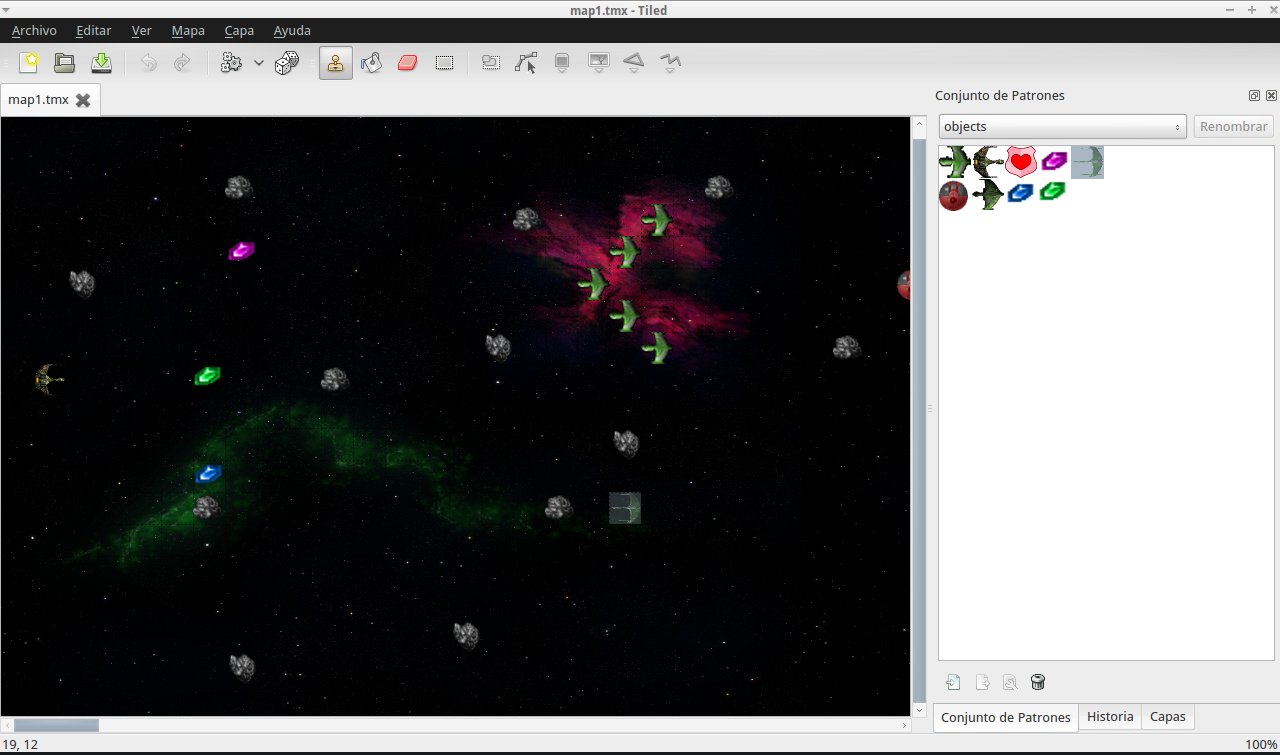
\includegraphics[width=\linewidth]{includes/images/tiled.png}
\caption{Captura de pantalla del programa de generación de mapas}
\label{fig:TiledScreenShoot}
\end{figure}

\section{Sistema de juego basado en nivel de salud y número de vidas}

Actualmente está implementado un sistema de juego basado en nivel de salud, que se decrementa con los disparos recibidos o en general colisiones y puede incrementarse al recoger objetos de salud, no está implementado un sistema basado en número de vidas, pero su implementación sería relativamente sencilla y abordable rapidamente.

\section{Desplegado de la aplicación sistemas soportados y sistemas objetivo}

Actualmente el juego se despliega sobre tres sistemas, Mac, windows y linux, para estos tres sistemas el juego es una simple aplicación de escritorio.Se detalla para cada plataforma:

\begin{itemize}

\item Mac: Tras el correcto empaquetado se proporciona un .app que tras instalarse da acceso al juego.

\item Windows:  Tras el correcto empaquetado se proporciona un .exe que es el ejecutable del juego.

\item Linux: Tras un simple empaquetado se proporciona un .love que ejecutado por la aplicacion para linux love2d ejecutará el juego.

\end{itemize}

Existe además un sistema de despliegue automático basado en un script shell que basicamente se encarga de las siguientes tareas:

\begin{itemize}

\item Empaquetado del juego para cada plataforma

\item Subir cada empaquetado a github en el repositorio llamado RenegadeKlingonDeploy: Para cada plataforma se sube sobre un branch independiente

\item Hacer merge entre los branches de cada plataforma y subir dicho merge sobre el branch master para ofrecer la posibilidad de descargar el juego para las tres plataformas a la vez.

\end{itemize}

Tener el sistema de despliegue automatizado supone una gran ventaja ya que si realizamos cualquier cambio sobre el juego podemos desplegar dicho cambio inmediatamente, y la gente que a partir de ese momento se descargue el juego tendra el último cambio que hemos añadido.

Migrar el juego a Mac y Windows ha sido relativamente sencillo, simplemente son cuestiones de como empaquetar el entregable final que maneja el script comentado anteriormente. Las siguientes plataformas objetivo son dispositivos móviles y desplegado directamente sobre web para ser jugado online, detallamos a continuación ciertas ideas técnicas sobre como llevar a cabo estas migraciones:

\begin{itemize}

\item Android: En principio, pensaba estudiar el proyecto love-native-android \url{https://github.com/hagish/love-native-android}. Muy probablemente habría que mejorar el juego en temas de resolución de pantalla y puede que aparecieran bugs al jugar sobre android. Además habría que estudiar temas de licencia y leer con detalle la licencia del proyecto love-native-android.

\item Iphone: Por el conocimiento que tengo hasta ahora no es técnicamente viable, no hay proyectos que migren automaticamente, y por las discusiones en foros hacer un proyecto a tal fin es una tarea muy compleja.Para llegar a Iphone podrían plantearse vias alternativas como jugar via web

\item Web: Existe un proyecto llamado love-webplayer \url{https://github.com/ghoulsblade/love-webplayer/wiki} que pretende ser un player de love2d sobre javascript, si ese proyecto funciona seria sencillo poner disponible el proyecto via web, también existe algun proyecto similar pero sobre html5, simplemente habria que estudiar estos proyectos y ver cual funciona mejor con el juego.

\end{itemize}
%\end{document} % Fin del documento